% ============================================================================
% CHAPTER 1: INTRODUCTION TO MACHINE LEARNING
% ============================================================================

\chapter{Introduction to Machine Learning}
\label{ch:introduction}

% ============================================================================
% OVERVIEW
% ============================================================================

\section{Chapter Overview}

Machine learning represents a paradigm shift in how we approach problem-solving with computers. This chapter introduces the fundamental concepts of machine learning, contrasts it with traditional programming approaches, and establishes the vocabulary and mental frameworks necessary for understanding the deeper concepts that follow.

\textbf{Learning Objectives:}
\begin{itemize}
    \item Understand the motivation behind machine learning
    \item Distinguish between traditional programming and machine learning paradigms
    \item Define representation learning and deep learning
    \item Learn the formal definition of machine learning (Tom Mitchell's definition)
    \item Identify different types of ML tasks, performance measures, and learning paradigms
    \item Understand the typical ML/DL pipeline
\end{itemize}

% ============================================================================
% THE DREAM: INTELLIGENT MACHINES
% ============================================================================

\section{The Dream of Intelligent Machines}

The aspiration to create machines that can think, reason, and learn like humans has driven researchers for decades. The fundamental question is: \textit{Can we somehow formalize thinking itself?} Can we create mathematical or algorithmic representations of the cognitive processes that humans perform naturally?

\begin{bluebox}[Historical Context: The Quest for Artificial Intelligence]
The dream of creating intelligent machines dates back centuries, but the formal field of Artificial Intelligence was established at the Dartmouth Conference in 1956. Early pioneers like Alan Turing, John McCarthy, and Marvin Minsky laid the groundwork for what would become one of the most transformative technologies of our time.

Turing proposed the famous ``Turing Test'' in 1950, asking whether a machine could exhibit intelligent behavior indistinguishable from a human. This question still resonates today as we witness large language models engaging in remarkably human-like conversations.
\end{bluebox}

% ============================================================================
% TRADITIONAL PROGRAMMING VS MACHINE LEARNING
% ============================================================================

\section{Traditional Programming vs Machine Learning}

\subsection{The Traditional Programming Paradigm}

In traditional programming, a human programmer writes explicit rules that the computer follows. The flow is:

\begin{center}
\begin{tikzpicture}[
    box/.style={draw, rounded corners, minimum width=2.5cm, minimum height=1cm, align=center, fill=gray!10},
    arrow/.style={-Stealth, thick}
]
    \node[box, fill=blue!20] (input) at (0,0) {Input\\Data};
    \node[box, fill=green!20] (program) at (4,0) {Hand-Designed\\Program};
    \node[box, fill=red!20] (output) at (8,0) {Output};
    
    \draw[arrow] (input) -- (program);
    \draw[arrow] (program) -- (output);
\end{tikzpicture}
\end{center}

\begin{examplebox}[Traditional Programming Example]
Consider sorting numbers. A programmer explicitly writes rules like:
\begin{enumerate}
    \item Compare adjacent elements
    \item If out of order, swap them
    \item Repeat until no swaps needed
\end{enumerate}
Every possible scenario must be anticipated and coded.
\end{examplebox}

\subsection{The Machine Learning Paradigm}

Machine learning inverts this approach. Instead of programming explicit rules, we provide \textit{examples} and let the algorithm discover patterns:

\begin{center}
\begin{tikzpicture}[
    box/.style={draw, rounded corners, minimum width=2.5cm, minimum height=1cm, align=center, fill=gray!10},
    arrow/.style={-Stealth, thick}
]
    \node[box, fill=blue!20] (input) at (0,0) {Input\\Data};
    \node[box, fill=orange!20] (output) at (4,0) {Expected\\Output};
    \node[box, fill=purple!20] (learning) at (2,-2) {Learning\\Algorithm};
    \node[box, fill=green!30] (program) at (2,-4) {Learned\\Program};
    
    \draw[arrow] (input) -- (learning);
    \draw[arrow] (output) -- (learning);
    \draw[arrow] (learning) -- (program);
\end{tikzpicture}
\end{center}

\begin{definitionbox}[Machine Learning]
Machine learning is the field of study that gives computers the ability to learn patterns from data without being explicitly programmed for each specific task. The computer discovers the ``program'' (the mapping from inputs to outputs) by analyzing examples.
\end{definitionbox}

\subsection{When Traditional Programming Fails}

Traditional rule-based programming works well for well-defined problems with clear logic. However, many real-world tasks are extremely difficult or impossible to define with explicit rules:

\begin{itemize}
    \item \textbf{Image Recognition}: How do you write rules to identify a cat in an image? Consider all possible poses, lighting conditions, occlusions, and cat breeds.
    \item \textbf{Speech Recognition}: The same word can sound vastly different based on accent, speed, pitch, and background noise.
    \item \textbf{Natural Language Understanding}: Language is ambiguous, context-dependent, and constantly evolving.
\end{itemize}

\begin{bluebox}[The Curse of Enumeration]
Consider the task of identifying a car in an image. One might attempt to define rules:
\begin{itemize}
    \item ``Look for four wheels''
    \item ``Check for a windshield''
    \item ``Identify the body shape''
\end{itemize}

But what about:
\begin{itemize}
    \item A car covered in snow (no visible wheels)?
    \item A car reflected in water?
    \item A sports car vs. an SUV vs. a vintage automobile?
    \item A car at an unusual angle?
\end{itemize}

The number of possible variations is virtually infinite. This is why \textbf{learning from examples} is more powerful than \textbf{enumerating rules}.
\end{bluebox}

% ============================================================================
% REPRESENTATION LEARNING
% ============================================================================

\section{From Features to Representations}

\subsection{Hand-Crafted Features (Classical ML)}

In classical machine learning, domain experts design \textit{features}---measurable properties of the data that are relevant to the task. The machine learning algorithm then learns a mapping from these features to the output.

\begin{center}
\begin{tikzpicture}[
    box/.style={draw, rounded corners, minimum width=2.8cm, minimum height=1cm, align=center},
    learned/.style={draw, rounded corners, minimum width=2.8cm, minimum height=1cm, align=center, fill=yellow!20, thick, dashed},
    arrow/.style={-Stealth, thick}
]
    \node[box, fill=blue!20] (input) at (0,0) {Input};
    \node[box, fill=gray!20] (features) at (3.5,0) {Hand-Designed\\Features};
    \node[learned] (mapping) at (7,0) {Learned\\Mapping};
    \node[box, fill=red!20] (output) at (10.5,0) {Output};
    
    \draw[arrow] (input) -- (features);
    \draw[arrow] (features) -- (mapping);
    \draw[arrow] (mapping) -- (output);
\end{tikzpicture}
\end{center}

\textbf{Example}: For classifying flowers (the Iris dataset):
\begin{itemize}
    \item Feature 1: Sepal length
    \item Feature 2: Sepal width
    \item Feature 3: Petal length
    \item Feature 4: Petal width
\end{itemize}

\subsection{Representation Learning}

\textbf{Representation learning} goes a step further: instead of relying on hand-crafted features, the algorithm learns the features (representations) themselves.

\begin{center}
\begin{tikzpicture}[
    box/.style={draw, rounded corners, minimum width=2.8cm, minimum height=1cm, align=center},
    learned/.style={draw, rounded corners, minimum width=2.8cm, minimum height=1cm, align=center, fill=yellow!20, thick, dashed},
    arrow/.style={-Stealth, thick}
]
    \node[box, fill=blue!20] (input) at (0,0) {Input};
    \node[learned] (features) at (3.5,0) {Learned\\Features};
    \node[learned] (mapping) at (7,0) {Learned\\Mapping};
    \node[box, fill=red!20] (output) at (10.5,0) {Output};
    
    \draw[arrow] (input) -- (features);
    \draw[arrow] (features) -- (mapping);
    \draw[arrow] (mapping) -- (output);
\end{tikzpicture}
\end{center}

\begin{bluebox}[The Power of Learned Representations]
Why is representation learning important?

\begin{enumerate}
    \item \textbf{Eliminates Domain Expertise Bottleneck}: Feature engineering requires deep domain knowledge. Representation learning can discover relevant features automatically.
    
    \item \textbf{Discovers Non-Obvious Patterns}: Humans might miss important features that the algorithm can discover.
    
    \item \textbf{Transfers Across Tasks}: Good representations learned for one task often help with related tasks.
\end{enumerate}
\end{bluebox}

% ============================================================================
% DEEP LEARNING
% ============================================================================

\section{Deep Learning: Hierarchical Representations}

\subsection{The Limitation of Single-Level Representations}

Consider the car recognition problem. The same car can appear very different under various conditions:
\begin{itemize}
    \item Different viewing angles
    \item Various lighting conditions
    \item Partial occlusion
    \item Different backgrounds
\end{itemize}

A single layer of learned features struggles to capture all these variations.

\subsection{The Deep Learning Approach}

\textbf{Deep learning} extends representation learning by learning \textit{multiple layers} of increasingly abstract representations:

\begin{center}
\begin{tikzpicture}[
    box/.style={draw, rounded corners, minimum width=2.2cm, minimum height=0.9cm, align=center},
    learned/.style={draw, rounded corners, minimum width=2.2cm, minimum height=0.9cm, align=center, fill=yellow!20, thick, dashed},
    arrow/.style={-Stealth, thick}
]
    \node[box, fill=blue!20] (input) at (0,0) {Input};
    \node[learned] (simple) at (2.5,0) {Simple\\Features};
    \node[learned] (complex1) at (5,0) {Higher-Level\\Features};
    \node[learned] (complex2) at (7.5,0) {...};
    \node[learned] (mapping) at (10,0) {Learned\\Mapping};
    \node[box, fill=red!20] (output) at (12.5,0) {Output};
    
    \draw[arrow] (input) -- (simple);
    \draw[arrow] (simple) -- (complex1);
    \draw[arrow] (complex1) -- (complex2);
    \draw[arrow] (complex2) -- (mapping);
    \draw[arrow] (mapping) -- (output);
\end{tikzpicture}
\end{center}

\subsection{Hierarchical Composition: The Image Example}

Consider how a deep learning system might process an image for face recognition:

\begin{center}
\begin{tikzpicture}[
    level/.style={draw, rounded corners, minimum width=3cm, minimum height=1.5cm, align=center, fill=blue!10},
    arrow/.style={-Stealth, thick, >=latex}
]
    \node[level, fill=blue!10] (l1) at (0,0) {\textbf{Layer 1}\\Edges\\(horizontal, vertical,\\diagonal lines)};
    \node[level, fill=blue!20] (l2) at (4,0) {\textbf{Layer 2}\\Contours\\(curves, shapes)};
    \node[level, fill=blue!30] (l3) at (8,0) {\textbf{Layer 3}\\Parts\\(eyes, nose, mouth)};
    \node[level, fill=blue!40] (l4) at (12,0) {\textbf{Layer 4}\\Objects\\(full face)};
    
    \draw[arrow] (l1) -- (l2);
    \draw[arrow] (l2) -- (l3);
    \draw[arrow] (l3) -- (l4);
\end{tikzpicture}
\end{center}

\begin{definitionbox}[Deep Learning]
\textbf{Deep learning} is a subset of machine learning that uses neural networks with multiple layers (depth $> 2$) to learn hierarchical representations of data. Each layer transforms the representation into something more abstract, eventually producing features suitable for the final task.

\textbf{Why ``Deep''?} The term refers to the depth of the network---the number of layers through which the data passes. Deeper networks can learn more complex, abstract representations.
\end{definitionbox}

\begin{bluebox}[The Book Analogy]
Consider how a book is constructed:
\begin{center}
Letters $\rightarrow$ Words $\rightarrow$ Sentences $\rightarrow$ Paragraphs $\rightarrow$ Chapters $\rightarrow$ Book
\end{center}

Deep learning operates similarly. At each layer:
\begin{itemize}
    \item Simple elements (letters/edges) combine to form
    \item More complex structures (words/contours), which combine to form
    \item Higher-level concepts (sentences/object parts), ultimately forming
    \item Complete understanding (chapters/full objects)
\end{itemize}

This \textbf{hierarchical composition} is key to why deep learning works so well.
\end{bluebox}

% ============================================================================
% THE AI LANDSCAPE
% ============================================================================

\section{The AI Landscape: AI, ML, and Deep Learning}

\subsection{The Relationship Between Terms}

\begin{center}
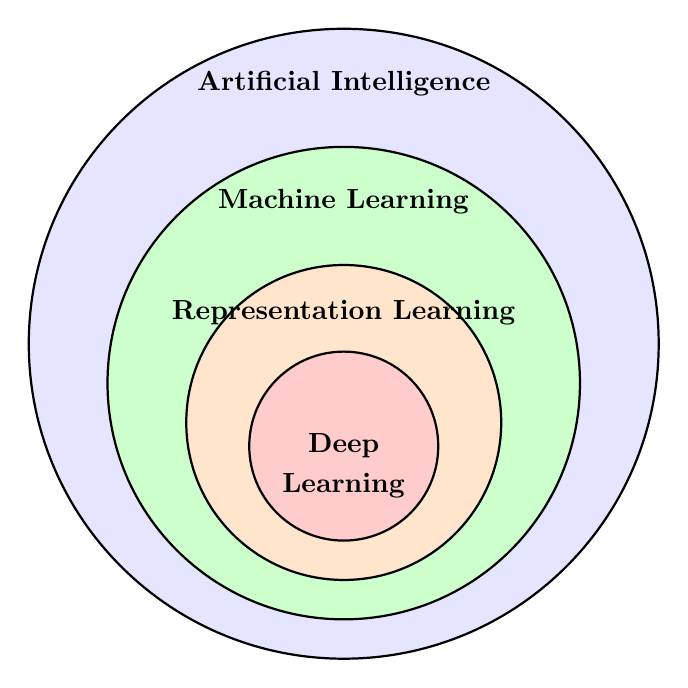
\begin{tikzpicture}
    % AI circle (outermost)
    \draw[thick, fill=blue!10] (0,0) circle (4cm);
    \node at (0,3.3) {\textbf{Artificial Intelligence}};
    
    % ML circle
    \draw[thick, fill=green!20] (0,-0.5) circle (3cm);
    \node at (0,1.8) {\textbf{Machine Learning}};
    
    % Representation Learning circle
    \draw[thick, fill=orange!20] (0,-1) circle (2cm);
    \node at (0,0.4) {\textbf{Representation Learning}};
    
    % Deep Learning circle (innermost)
    \draw[thick, fill=red!20] (0,-1.3) circle (1.2cm);
    \node at (0,-1.3) {\textbf{Deep}};
    \node at (0,-1.8) {\textbf{Learning}};
\end{tikzpicture}
\end{center}

\begin{itemize}
    \item \textbf{Artificial Intelligence (AI)}: The broadest category---any system that exhibits intelligent behavior. This includes rule-based systems, expert systems, and learning-based approaches.
    
    \item \textbf{Machine Learning (ML)}: A subset of AI where systems learn patterns from data rather than being explicitly programmed.
    
    \item \textbf{Representation Learning}: A subset of ML where the system learns the features/representations of data automatically.
    
    \item \textbf{Deep Learning (DL)}: A subset of representation learning using multi-layered neural networks to learn hierarchical representations.
\end{itemize}

\subsection{A Summary Diagram}

The evolution from rule-based to deep learning systems:

\begin{center}
\renewcommand{\arraystretch}{1.5}
\begin{tabular}{|c|c|c|c|c|}
\hline
\textbf{Paradigm} & \textbf{Input} & \textbf{Features} & \textbf{Mapping} & \textbf{Output} \\ \hline
Rule-based & Given & Hand-designed & Hand-designed & $\checkmark$ \\ \hline
Classical ML & Given & Hand-designed & \colorbox{yellow!30}{Learned} & $\checkmark$ \\ \hline
Rep. Learning & Given & \colorbox{yellow!30}{Learned} & \colorbox{yellow!30}{Learned} & $\checkmark$ \\ \hline
Deep Learning & Given & \colorbox{yellow!30}{\begin{tabular}{c}Learned\\(Hierarchical)\end{tabular}} & \colorbox{yellow!30}{Learned} & $\checkmark$ \\ \hline
\end{tabular}
\end{center}

\begin{bluebox}[Historical Note: The AI Winters]
The history of AI has seen periods of great hope followed by disappointment:

\textbf{1950s-1960s}: Early enthusiasm. Researchers promised thinking machines were imminent.

\textbf{1970s (First AI Winter)}: The Perceptron was shown unable to solve XOR. Funding dried up.

\textbf{1980s}: Expert systems revival, multi-layer networks developed.

\textbf{Late 1980s-1990s (Second AI Winter)}: Expert systems proved brittle and hard to maintain.

\textbf{2012-Present}: Deep learning renaissance. AlexNet won ImageNet, GPT and large language models emerged.

The field underwent multiple name changes: Cybernetics $\rightarrow$ Connectionism $\rightarrow$ Neural Networks $\rightarrow$ Machine Learning $\rightarrow$ Deep Learning, partly to escape the stigma of previous ``AI winters.''
\end{bluebox}

% ============================================================================
% FORMAL DEFINITION OF LEARNING
% ============================================================================

\section{The Formal Definition of Learning}

\subsection{Tom Mitchell's Definition}

The computer scientist Tom Mitchell provided one of the most widely cited definitions of machine learning:

\begin{theorembox}[Tom Mitchell's Definition of Learning (1997)]
A computer program is said to \textbf{learn} from experience $\mathbf{E}$ with respect to some class of tasks $\mathbf{T}$ and performance measure $\mathbf{P}$, if its performance at tasks in $\mathbf{T}$, as measured by $\mathbf{P}$, improves with experience $\mathbf{E}$.
\end{theorembox}

This definition identifies three essential components of any learning system:

\begin{enumerate}
    \item \textbf{Task (T)}: What the system is trying to accomplish
    \item \textbf{Performance Measure (P)}: How we quantify success
    \item \textbf{Experience (E)}: The data the system learns from
\end{enumerate}

\subsection{Example: Learning to Play Chess}

\begin{itemize}
    \item \textbf{Task (T)}: Play chess (make legal moves, try to win)
    \item \textbf{Performance (P)}: Win rate against opponents
    \item \textbf{Experience (E)}: Playing games, analyzing past games
\end{itemize}

If, after playing many games, the win rate improves, then the program has \textit{learned}.

\subsection{Example: Email Spam Classification}

\begin{itemize}
    \item \textbf{Task (T)}: Classify emails as spam or not-spam
    \item \textbf{Performance (P)}: Accuracy (percentage correctly classified)
    \item \textbf{Experience (E)}: A dataset of labeled emails
\end{itemize}

% ============================================================================
% MACHINE LEARNING TASKS
% ============================================================================

\section{Types of Machine Learning Tasks}

\subsection{Classification}

The task of assigning an input to one of $k$ discrete categories.

\begin{definitionbox}[Classification]
A function $f: \R^n \rightarrow \{1, 2, \ldots, k\}$ that maps an $n$-dimensional feature vector to one of $k$ class labels.
\end{definitionbox}

\textbf{Examples}:
\begin{itemize}
    \item Image classification (cat vs. dog)
    \item Spam detection (spam vs. not-spam)
    \item Medical diagnosis (disease A, B, C, or healthy)
    \item Handwritten digit recognition (0-9)
\end{itemize}

\subsection{Regression}

The task of predicting a continuous numerical value.

\begin{definitionbox}[Regression]
A function $f: \R^n \rightarrow \R$ that maps an $n$-dimensional feature vector to a real-valued output.
\end{definitionbox}

\textbf{Examples}:
\begin{itemize}
    \item Stock price prediction
    \item House price estimation
    \item Temperature forecasting
    \item Age estimation from photographs
\end{itemize}

\subsection{Other Important Tasks}

\begin{itemize}
    \item \textbf{Classification with Missing Values}: Classification when some features are unavailable
    \item \textbf{Transcription}: Converting unstructured data to structured form (e.g., speech-to-text, image captioning)
    \item \textbf{Machine Translation}: Converting text from one language to another
    \item \textbf{Structured Output}: Outputs with relationships between elements (e.g., parsing sentences)
    \item \textbf{Anomaly Detection}: Identifying unusual patterns (e.g., fraud detection)
    \item \textbf{Synthesis/Sampling}: Generating new data similar to training data (e.g., image generation)
    \item \textbf{Imputation}: Filling in missing values
    \item \textbf{Denoising}: Removing noise from signals (e.g., image deblurring)
    \item \textbf{Density Estimation}: Learning the probability distribution of data
\end{itemize}

% ============================================================================
% PERFORMANCE MEASURES
% ============================================================================

\section{Performance Measures}

Performance measures (metrics) quantify how well a model performs its task.

\subsection{Common Metrics}

\begin{itemize}
    \item \textbf{Accuracy}: 
    \[
    \text{Accuracy} = \frac{\text{Correct Predictions}}{\text{Total Predictions}}
    \]
    
    \item \textbf{Error Rate}: $1 - \text{Accuracy}$
    
    \item \textbf{Precision}: Of all positive predictions, how many were correct?
    \[
    \text{Precision} = \frac{\text{True Positives}}{\text{True Positives} + \text{False Positives}}
    \]
    
    \item \textbf{Recall}: Of all actual positives, how many were detected?
    \[
    \text{Recall} = \frac{\text{True Positives}}{\text{True Positives} + \text{False Negatives}}
    \]
    
    \item \textbf{F1 Score}: Harmonic mean of precision and recall
    \[
    F_1 = 2 \cdot \frac{\text{Precision} \cdot \text{Recall}}{\text{Precision} + \text{Recall}}
    \]
    
    \item \textbf{AUC-ROC}: Area Under the Receiver Operating Characteristic Curve
\end{itemize}

\begin{bluebox}[Choosing the Right Metric]
The choice of metric depends on the problem:
\begin{itemize}
    \item For balanced datasets: Accuracy often suffices
    \item For imbalanced data: Precision, Recall, F1 are more informative
    \item For ranking problems: AUC-ROC is preferred
    \item For regression: Mean Squared Error (MSE), Mean Absolute Error (MAE)
\end{itemize}

In fraud detection, for example, accuracy might be misleading---99\% accuracy could mean missing all fraud cases if fraud is only 1\% of transactions!
\end{bluebox}

% ============================================================================
% LEARNING PARADIGMS
% ============================================================================

\section{Learning Paradigms: The Experience}

How does a machine learning system gain ``experience''? This depends on the type of data and feedback available.

\subsection{Supervised Learning}

The algorithm learns from labeled examples.

\begin{definitionbox}[Supervised Learning]
Given a dataset $\mathcal{D} = \{(\vect{x}_1, y_1), (\vect{x}_2, y_2), \ldots, (\vect{x}_n, y_n)\}$ where each $\vect{x}_i$ is a feature vector and $y_i$ is the corresponding label, learn a function $f$ that maps inputs to outputs.
\end{definitionbox}

\textbf{Examples}: Classification, regression

\subsection{Unsupervised Learning}

The algorithm learns patterns without labeled outputs.

\begin{definitionbox}[Unsupervised Learning]
Given a dataset $\mathcal{D} = \{\vect{x}_1, \vect{x}_2, \ldots, \vect{x}_n\}$ (no labels), discover the underlying structure or patterns in the data.
\end{definitionbox}

\textbf{Examples}: Clustering, dimensionality reduction, density estimation

\subsection{Semi-Supervised Learning}

Some examples are labeled, others are not. This is common in practice (labeling is expensive).

\subsection{Reinforcement Learning}

An agent learns by interacting with an environment and receiving rewards.

\begin{definitionbox}[Reinforcement Learning]
An \textbf{agent} takes \textbf{actions} in an \textbf{environment}, transitioning between \textbf{states}. Each transition yields a \textbf{reward}. The agent learns a \textbf{policy} that maximizes cumulative reward.
\end{definitionbox}

Key concepts:
\begin{itemize}
    \item \textbf{Exploration}: Trying new actions to discover their effects
    \item \textbf{Exploitation}: Using known good actions to maximize reward
    \item \textbf{Exploration-Exploitation Trade-off}: Balancing discovery with optimization
\end{itemize}

\textbf{Examples}:
\begin{itemize}
    \item AlphaGo: Learning to play the game Go
    \item Robotic control: Learning to walk
    \item RLHF (Reinforcement Learning from Human Feedback): Training ChatGPT
\end{itemize}

% ============================================================================
% THE ML PIPELINE
% ============================================================================

\section{The Machine Learning Pipeline}

A typical ML/DL project follows a structured pipeline:

\begin{center}
\begin{tikzpicture}[
    box/.style={draw, rounded corners, minimum width=2cm, minimum height=1.2cm, align=center, fill=blue!10},
    arrow/.style={-Stealth, thick}
]
    % Row 1
    \node[box, fill=blue!20] (p1) at (0,0) {\textbf{1.} Problem\\Definition};
    \node[box, fill=green!20] (p2) at (3.5,0) {\textbf{2.} Data\\Collection};
    \node[box, fill=yellow!20] (p3) at (7,0) {\textbf{3.} Data\\Preprocessing};
    \node[box, fill=orange!20] (p4) at (10.5,0) {\textbf{4.} Model\\Selection};
    
    % Row 2
    \node[box, fill=red!20] (p5) at (0,-3) {\textbf{5.} Model\\Training};
    \node[box, fill=purple!20] (p6) at (3.5,-3) {\textbf{6.} Model\\Evaluation};
    \node[box, fill=cyan!20] (p7) at (7,-3) {\textbf{7.} Model\\Testing};
    \node[box, fill=gray!30] (p8) at (10.5,-3) {\textbf{8.} Deployment\\Monitoring};
    
    \draw[arrow] (p1) -- (p2);
    \draw[arrow] (p2) -- (p3);
    \draw[arrow] (p3) -- (p4);
    \draw[arrow] (p4) -- (p4 |- 0,-1.5) -- (p5 |- 0,-1.5) -- (p5);
    \draw[arrow] (p5) -- (p6);
    \draw[arrow] (p6) -- (p7);
    \draw[arrow] (p7) -- (p8);
\end{tikzpicture}
\end{center}

\subsection{Step 1: Problem Definition}
\begin{itemize}
    \item Define the task (classification, regression, etc.)
    \item Clarify the objective (what does success look like?)
    \item Understand the business or scientific context
\end{itemize}

\subsection{Step 2: Data Collection}
\begin{itemize}
    \item Identify data sources (databases, APIs, sensors, web scraping)
    \item Gather relevant data
    \item Format data appropriately (CSV, JSON, images, etc.)
\end{itemize}

\subsection{Step 3: Data Preprocessing}

\begin{itemize}
    \item \textbf{Data Cleaning}: Handle missing values, remove duplicates, fix inconsistencies
    \item \textbf{Feature Engineering}: Create new features, encode categorical variables, scale/normalize
    \item \textbf{Data Splitting}: Divide into training, validation, and test sets
    \item \textbf{Data Augmentation}: Artificially expand the dataset (e.g., flip images, add noise)
\end{itemize}

\begin{bluebox}[Garbage In, Garbage Out]
Data preprocessing is often where 60\% or more of project time is spent. The quality of your data directly determines the quality of your model. No amount of sophisticated algorithms can compensate for poor data.
\end{bluebox}

\subsection{Step 4: Model Selection/Design}

\begin{itemize}
    \item Choose appropriate algorithms (Decision Trees, Neural Networks, SVMs, etc.)
    \item Design architecture (for deep learning: number of layers, neurons, etc.)
\end{itemize}

\subsection{Step 5: Model Training}

\begin{itemize}
    \item Choose a loss function (how to measure error)
    \item Select an optimizer (SGD, Adam, etc.)
    \item Fit the model to training data
    \item Use batching for large datasets
\end{itemize}

\subsection{Step 6: Model Evaluation}

\begin{itemize}
    \item Compute performance metrics on validation set
    \item Perform cross-validation
    \item Hyperparameter tuning (learning rate, regularization, architecture choices)
\end{itemize}

\subsection{Step 7: Model Testing}

\begin{itemize}
    \item Evaluate on held-out test set
    \item Check for overfitting (memorizing training data) or underfitting (poor performance)
\end{itemize}

\subsection{Step 8: Deployment and Monitoring}

\begin{itemize}
    \item Export the model
    \item Deploy via APIs (Flask, FastAPI)
    \item Monitor performance in production
    \item Retrain as needed (handle model drift)
\end{itemize}

\begin{examplebox}[Fraud Detection Pipeline]
\textbf{Problem}: Detect fraudulent credit card transactions

\textbf{Data Collection}: Obtain transaction records from banks (customer ID, amount, time, merchant, etc.)

\textbf{Preprocessing}: Handle missing timestamps, create features (transaction frequency, deviation from average amount), encode merchant categories

\textbf{Model}: XGBoost or deep neural network

\textbf{Training}: Binary cross-entropy loss, Adam optimizer

\textbf{Evaluation}: Precision, Recall, F1 Score (accuracy alone is misleading due to class imbalance)

\textbf{Deployment}: Real-time API that scores each transaction

\textbf{Monitoring}: Track model drift as fraudsters adapt their strategies
\end{examplebox}

% ============================================================================
% WHY NOW?
% ============================================================================

\section{Why Machine Learning is Thriving Now}

Many core algorithms (including backpropagation) were developed in the 1970s-1980s. So why has ML/DL taken off only recently?

\subsection{The Three Pillars}

\begin{center}
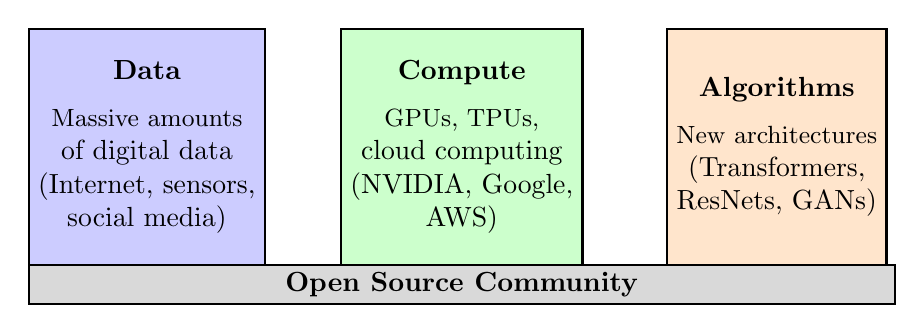
\begin{tikzpicture}[
    pillar/.style={draw, thick, minimum width=2.5cm, minimum height=3cm, fill=blue!10, align=center}
]
    \node[pillar, fill=blue!20] (p1) at (0,0) {\textbf{Data}\\[5pt]\small Massive amounts\\of digital data\\(Internet, sensors,\\social media)};
    \node[pillar, fill=green!20] (p2) at (4,0) {\textbf{Compute}\\[5pt]\small GPUs, TPUs,\\cloud computing\\(NVIDIA, Google,\\AWS)};
    \node[pillar, fill=orange!20] (p3) at (8,0) {\textbf{Algorithms}\\[5pt]\small New architectures\\(Transformers,\\ResNets, GANs)};
    
    % Base
    \draw[thick, fill=gray!30] (-1.5,-2) rectangle (9.5,-1.5);
    \node at (4,-1.75) {\textbf{Open Source Community}};
\end{tikzpicture}
\end{center}

\begin{enumerate}
    \item \textbf{Data}: The internet age has produced unprecedented amounts of data. Web scraping, social media, IoT sensors---data is everywhere.
    
    \item \textbf{Compute Power}: GPUs (Graphics Processing Units) enable massive parallelization. What took weeks now takes hours. NVIDIA's GPUs have become the ``shovels in the AI gold rush.''
    
    \item \textbf{Algorithmic Advances}: New architectures like Transformers, ResNets, and techniques like dropout and batch normalization have overcome previous limitations.
    
    \item \textbf{Open Source}: Frameworks like TensorFlow, PyTorch, and pre-trained models allow rapid experimentation. The community shares knowledge freely.
\end{enumerate}

\begin{bluebox}[The Shovel Sellers in a Gold Rush]
There's a famous business principle: ``In a gold rush, don't mine for gold---sell shovels.'' NVIDIA exemplified this perfectly. While companies race to build the best AI models, NVIDIA provides the hardware (GPUs) that everyone needs. This is why NVIDIA's valuation skyrocketed during the AI boom.
\end{bluebox}

% ============================================================================
% CHAPTER SUMMARY
% ============================================================================

\section{Chapter Summary}

\begin{itemize}
    \item \textbf{Machine Learning} is a paradigm where computers learn patterns from data rather than being explicitly programmed.
    
    \item \textbf{Representation Learning} allows algorithms to discover the features themselves, rather than relying on hand-crafted features.
    
    \item \textbf{Deep Learning} uses multiple layers to learn hierarchical representations, enabling handling of complex, high-dimensional data.
    
    \item Tom Mitchell's definition formalizes learning: improvement on task $T$ with respect to measure $P$ through experience $E$.
    
    \item ML tasks include classification, regression, transcription, translation, anomaly detection, and more.
    
    \item Learning paradigms: supervised (labeled data), unsupervised (no labels), semi-supervised (partial labels), reinforcement (rewards).
    
    \item The ML pipeline: Problem Definition $\rightarrow$ Data Collection $\rightarrow$ Preprocessing $\rightarrow$ Model Selection $\rightarrow$ Training $\rightarrow$ Evaluation $\rightarrow$ Testing $\rightarrow$ Deployment.
    
    \item ML/DL is thriving due to abundant data, powerful compute, algorithmic innovations, and open-source culture.
\end{itemize}
